\documentclass[12pt, titlepage]{article}

\usepackage{booktabs}
\usepackage{tabularx}
\usepackage{graphicx}
\usepackage{hyperref}
\hypersetup{
    colorlinks,
    citecolor=black,
    filecolor=black,
    linkcolor=red,
    urlcolor=blue
}
\usepackage[round]{natbib}

\title{SE 3XA3: Test Report\\PocketSaver}

\author{Team 12
		\\ Mevin Mathew, mathem1
		\\ Shalmi Patel, patels19
		\\ Diya Mathews, mathewsd
}

\date{\today}

%% Comments

\usepackage{color}

\newif\ifcomments\commentstrue

\ifcomments
\newcommand{\authornote}[3]{\textcolor{#1}{[#3 ---#2]}}
\newcommand{\todo}[1]{\textcolor{red}{[TODO: #1]}}
\else
\newcommand{\authornote}[3]{}
\newcommand{\todo}[1]{}
\fi

\newcommand{\wss}[1]{\authornote{blue}{SS}{#1}}
\newcommand{\ds}[1]{\authornote{red}{DS}{#1}}
\newcommand{\mj}[1]{\authornote{red}{MSN}{#1}}
\newcommand{\mh}[1]{\authornote{red}{MH}{#1}}
\newcommand{\cm}[1]{\authornote{red}{CM}{#1}}


% team members should be added for each team, like the following
% all comments left by the TAs or the instructor should be addressed
% by a corresponding comment from the Team

\newcommand{\tm}[1]{\authornote{magenta}{Team}{#1}}


\begin{document}

\maketitle

\pagenumbering{roman}
\tableofcontents
\listoftables
\listoffigures

\begin{table}[bp]
\caption{\bf Revision History}
\begin{tabularx}{\textwidth}{p{3cm}p{2cm}X}
\toprule {\bf Date} & {\bf Version} & {\bf Notes}\\
\midrule
12/04/2017 & 1.0 & Initial\\
12/06/2017 & 1.1 & Rev1\\
\bottomrule
\end{tabularx}
\end{table}

\newpage

\pagenumbering{arabic}

This document describes the results of all testing done for PocketSaver based on the Test Plan we documented.

\section{Functional Requirements Evaluation}
\subsubsection{Input}

\begin{enumerate}

\item{Test User Input\\} \label{I1}
inputTest-id1 : Testing if user’s input is being received
\newline
Type: Functional, Dynamic, Automatic
\newline
Initial State: Application is on the enter transaction page
\newline
Input/Condition: User inputs their transaction details and clicks Enter
\newline
Expected Output/Result: The transaction should update the database 
\newline
Actual Output/Result: The transaction is updated on the database 
\newline
Result: Unit Test Passed

					
\item{Test Entry Modification\\} \label{I2}
inputTest-id2 : Testing if user is able to modify entries
\newline
Type: Functional, Dynamic, Automatic
\newline
Initial State: Database has at least one transaction
\newline
Input/Condition: User selects an existing transaction and modifies a parameter
\newline
Expected Output/Result: Modified transaction should update according to the modifications in the database
\newline
Actual Output/Result: The modified transaction is correctly updated on the database 
\newline
Result: Unit Test Passed

\item{Test Entry Deletion\\}\label{I3}
inputTest-id3 : Testing if user is able to delete entries
\newline
Type: Functional, Dynamic
\newline
Initial State: Database has at least one transaction
\newline
Input/Condition: User selects an existing transaction and deletes it
\newline
Expected Output/Result: Deleted transaction should not appear within database
\newline
Actual Output/Result: The deleted transaction is deleted on the database 
\newline
Result: Unit Test Passed

\item{Set monthly budget}\label{I4}
inputTest-id4 : Testing if user can set monthly budget
\newline
Type: Functional, Dynamic, Manual
\newline
Initial State: no budget set
\newline
Input/Condition: User enters a numerical value
\newline
Expected Output/Result: budget set, StorageSV is updated
\newline
Actual Output/Result: The budget is set and StorageSV is updated
\newline
Result: Manual Test Passed

\item{View monthly expenses}\label{I5}
inputTest-id5 : Select month to view expenses.
\newline
Type: Functional, Dynamic, Manual 
\newline
Initial State: 'select one of the following options' is displayed 
\newline
Input/Condition: User selects month
\newline
Expected Output/Result: Month's total expense is displayed
\newline
Actual Output/Result: Correct total expense is displayed
\newline
Result: Manual Test Passed
\end{enumerate}

\subsubsection{Application Output}\label{A1}
\begin{enumerate}
\item{Test delay of Cumulative Amount Spent }
\newline
outputTest-id1 : Testing if the total amount spent is up-to-date and has no delay
\newline
Type: Functional, Dynamic
\newline
Initial State: Database has at least one transaction
\newline
Input/Condition: User enters a new transaction on current date
\newline
Expected Output/Result: Entered transaction should appear in database and total amount spent today should be incremented.
\newline
Actual Output/Result: The entered transaction is present on the database and daily amount is incremented
\newline
Result: Unit Test Passed

\item{Testing Transaction List Page}\label{A2}
\newline
outputTest-id2 : Testing if the transaction page is up-to-date and has no delay
\newline
Type: Functional, Dynamic, Automatic
\newline
Initial State: Database has at least one transaction
\newline
Input/Condition: User enters a new transaction
\newline
Expected Output/Result: Entered transaction should appear in database and transaction list view
\newline
Actual Output/Result: The entered transaction is present on the database and transaction list view
\newline
Result: Unit Test Passed

\item{View daily expenses}\label{A3}
outputTest-id3 : Display current days' expenses
\newline
Type: Functional, Dynamic, Manual 
\newline
Initial State: 'select one of the following options' is displayed 
\newline
Input/Condition: User selects 'Daily'
\newline
Expected Output/Result: 'Daily' total expense is displayed
\newline
Actual Output/Result: The current days' expense is correctly displayed
\newline
Result: Unit Test Passed

\item{Display current budget}\label{A4}
outputTest-id4 : Display current budget
\newline
Type: Functional, Dynamic, Manual 
\newline
Initial State: No budget is entered
\newline
Input/Condition: User inputed numerical value into textbox
\newline
Expected Output/Result: Inputted budget value should be shown to user
\newline
Actual Output/Result: Current budget is displayed correctly
\newline
Result: Unit Test Passed
\end{enumerate}

\section{Nonfunctional Requirements Evaluation}
The nonfunction requirements were tested using a combination of manual testing, the usabilty survey we referenced in the test plan, and the feedback from the inlab presentation. Based on the feedback from the survey and inlab presentation, we made some modifications to our project and added a couple of features to better improve out application.

\subsection{Survey Questions}
 \label{survey:1}
Please provide a rating from 1 to 5 for the following statements (1 - Strongly Disagree, 2 - Disagree, 3 - Neutral, 4 - Agree, 5 - Strongly Agree) : 
\begin{enumerate}

\item The application is easy to navigate and easy to use. \label{question:q0}
\item The colour scheme is visually appealing.\label{question:q1}
\item Entering/modifying/deleting transactions are reflected on the total amount spent with little to no delay\label{question:q2}
\item Entering/modifying/deleting transactions are reflected on the transaction page with little to no delay\label{question:q3}
\item The application runs smoothly and with minimal wait/loading time.\label{question:q5}
\item I was comfortable with entering all information that the application asked me to.\label{question:q6}
\item Please provide detailed answers for the following questions (point-form is acceptable)\label{question:q7}
\item Does the application run smoothly on your device? Please indicate the device you used.\label{question:q8}
\item Were you offended by anything in this game? Please provide details\label{question:q9}
\item Is there anything you feel is missing or could be improved in this application?\label{question:q10}
\end{enumerate}

\subsubsection{Look and Feel}
\begin{enumerate}
\item{lookTest-id1\\}
lookTest-id1 : This will be tested by survey question ~\ref{Q3} and ~\ref{Q2} and ~\ref{Q8}
\newline
	Expected Result: An average of 90\% rating (4.5/5)
\newline
	Actual Result: Test Passed (Q3: 18/20 * 100\% = 90\%, 20/20 * 100\% = 100\%)
\end{enumerate}

\subsubsection{Usability and Humanity Requirements}
\begin{enumerate}
\item{usabilityTest-id1\\}
usabilityTest-id1 : This will be tested by survey question ~\ref{Q1} and ~\ref{Q2}
\newline
	Expected Result: An average of 90\% rating (4.5/5)
\newline
	Actual Result: Test Passed (Q1: 19/20 * 100\% = 95\%, Q2: 18/20 * 100\% = 90\%)

\item{usabilityTest-id2\\}
usabilityTest-id2 : This will be tested by survey question ~\ref{Q5}
\newline
	Expected Result: An average of 90\% rating (4.5/5)
\newline
	Actual Result: Test Passed (20/20 * 100\% = 100\%)
\end{enumerate}

\subsubsection{Performance Requirements}
\begin{enumerate}
\item{performanceTest-id1\\}
performanceTest-id1 : This will be tested by survey question ~\ref{Q4}
\newline
	Expected Result: An average of 90\% rating (4.5/5)
\newline
	Actual Result: Test Passed (19/20 * 100\% = 95\%)

\item{performanceTest-id2\\}
performanceTest-id2 : This will be tested by survey question ~\ref{Q5}
\newline
	Expected Result: An average of 90\% rating (4.5/5)
\newline
	Actual Result: Test Passed (20/20 * 100\% = 100\%)
\end{enumerate}

\subsubsection{Legal Requirements}
\begin{enumerate}
\item{legalTest-id1\\}
legalTest-id1 : This will be tested by survey question ~\ref{Q9}
\newline
	Expected Result: An average of 90\% of surveys say no
\newline
	Actual Result: Test Passed (20/20 * 100\% = 100\%)
\end{enumerate}

\subsubsection{Security Requirements}
\begin{enumerate}
\item{securityTest-id1\\}
securityTest-id1 : This will be tested by survey question ~\ref{Q6}
\newline
Expected Result: An average of 90\% of surveys say no
\newline
	Actual Result: Test Passed (18/20 * 100\% = 90\%)
\end{enumerate}

\subsubsection{Additional Suggestions from the Survey and inLab Feedback}
\begin{itemize}
\item {Add a today button to make it easier to enter todays date when entering a transaction.}
\item{A graph implementation to view monthly transaction}
\item{An overview of multiple months}
\item{Filter through transaction list page}
\end{itemize}

\section{Comparison to Existing Implementation}	
As we strived to accomplish, we created a smoother user interface than the existing implementation, CoCoin. PocketSaver uses an online database rather than a local one like CoCoin to ensure data integrity and save space on the user's local device. Another obstacle we had to over come was the language barrier, CoCoin was written in Mandrian, making it very difficult for us to follow along the project.

\section{Unit Testing}
Unit Testing was completed using the Visual Studios Testing Framework. The tests are located in the src directory as its own solution. There were 4 tests for the API service and 3 tests for the homepage view model. When running the unit tests, it is important to run the homepage view model tests before the API service because the API service generates new data which the homepage view model unit tests are not expecting. Therefore causing the homepage view model to fail even if its functionality is correct.
\begin{figure}[ht]
\centering
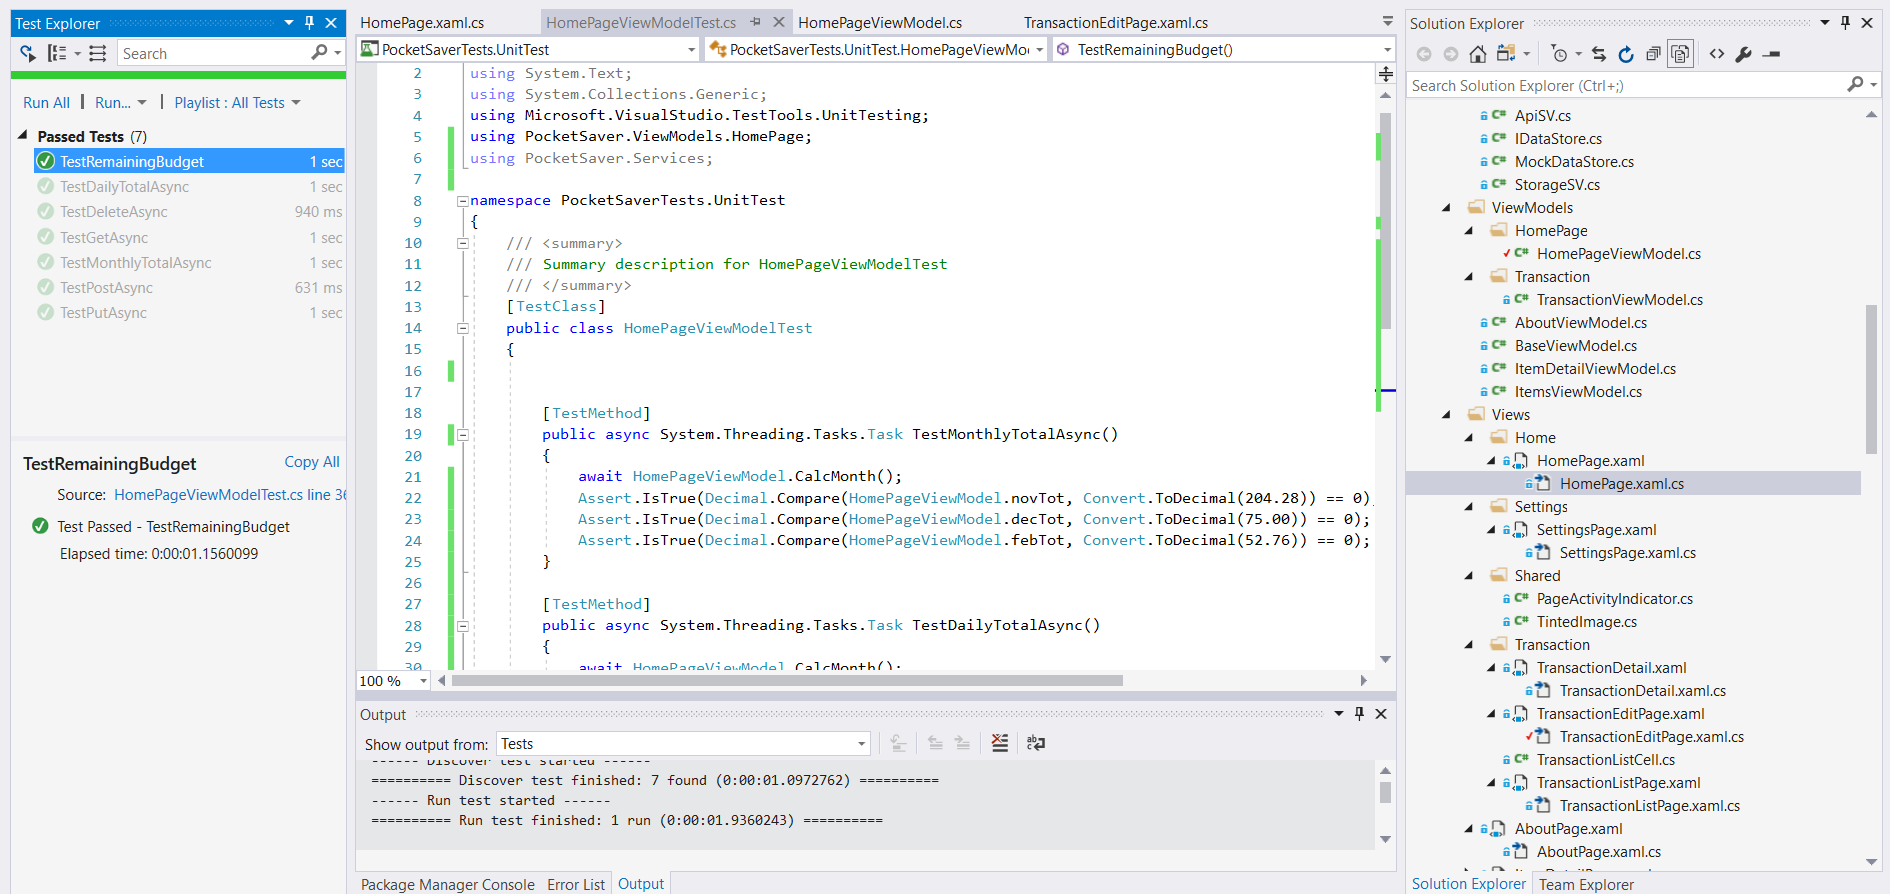
\includegraphics[width=0.7\textwidth]{UnitTesting.png}
\caption{Sample of the Unit Testing in Visual Studios}
\end{figure}

\section{Changes Due to Testing}
After conducting the non functional testing, we created a today button for easier use of the entering a transaction function of the applicaiton. We also fixed a few bugs that those who took our survey caught. We ensured that the navagation between the pages was correct and smooth. Taking into account the feedback from our tests, we were able to improve our application.

\section{Automated Testing}
Automated Testing was implemented using the Visual Studios Testing Framework as mentioned above. The automated testing was implementing to ensure the API calls to the database were working. This is the core of the application since without this none of the data would be saved and nothing else would work. Therefore ensuring the API calls were working was very important.

\section{Trace to Requirements}
The tables are found at the appendix at Table \ref{TraceFR} and Table \ref{TraceNFR}.

\section{Trace to Modules}		
The tables are found at the appendix at Table \ref{ModuleTraceFR}.

\section{Code Coverage Metrics}
For our application, every testcase passed, through both unit testing and manual testing. During testing both functional and non-functional requirements were tested, with normal cases and edge cases. The application has a smooth user interface, there for it was easy to validate functionality through a usability survey (inserted in this document) where targeted users tested the application. Therefore, our goal for 90\% coverage metric was reached.

\section{Appendix}
\begin{figure}[h]
\centering
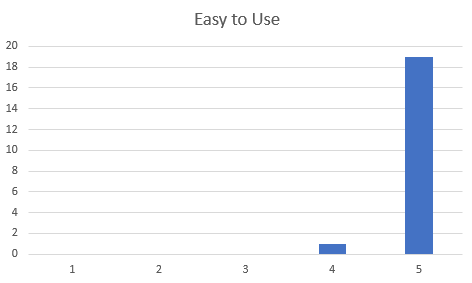
\includegraphics[width=0.7\textwidth]{Question1.png}
\caption{Results of Question 1 of the Survey}
\label{Q1}
\end{figure}

\begin{figure}[h]
\centering
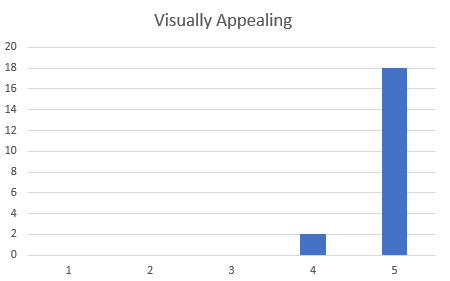
\includegraphics[width=0.7\textwidth]{Question2.png}
\caption{Results of Question 2 of the Survey}
\label{Q2}
\end{figure}

\begin{figure}[h]
\centering
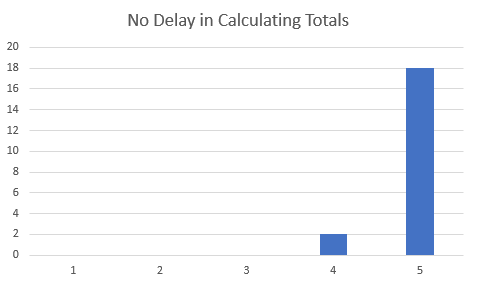
\includegraphics[width=0.7\textwidth]{Question3.png}
\caption{Results of Question 3 of the Survey}
\label{Q3}
\end{figure}

\begin{figure}[h]
\centering
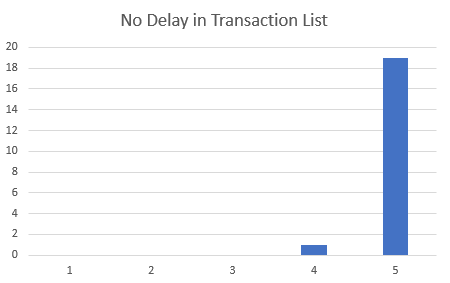
\includegraphics[width=0.7\textwidth]{Question4.png}
\caption{Results of Question 4 of the Survey}
\label{Q4}
\end{figure}
\clearpage

\begin{figure}[h]
\centering
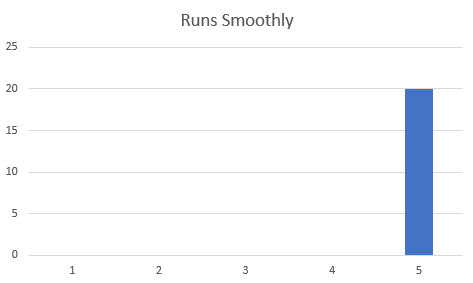
\includegraphics[width=0.7\textwidth]{Question5.png}
\caption{Results of Question 5 of the Survey}
\label{Q5}
\end{figure}

\begin{figure}[h]
\centering
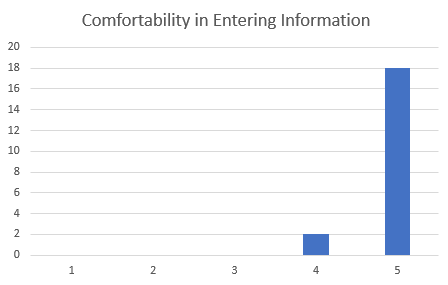
\includegraphics[width=0.7\textwidth]{Question6.png}
\caption{Results of Question 6 of the Survey}
\label{Q6}
\end{figure}

\begin{figure}[h]
\centering
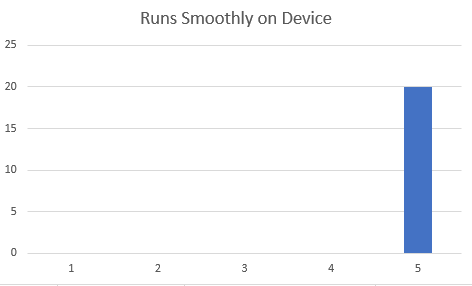
\includegraphics[width=0.7\textwidth]{Question8.png}
\caption{Results of Question 8 of the Survey}
\label{Q8}
\end{figure}

\begin{figure}[h]
\centering
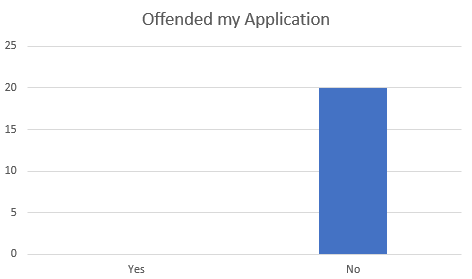
\includegraphics[width=0.7\textwidth]{Question9.png}
\caption{Results of Question 9 of the Survey}
\label{Q9}
\end{figure}

\begin{table}[ht]
\caption{\bf Trace to Funcitonal Requirements}
\label{TraceFR}
\begin{tabularx}{\textwidth}{p{5cm}p{8cm}}
\toprule {\bf TestID} & {\bf Functional Requirements ID}\\
\midrule
inputTest-id\ref{I1} & Functional Requirement 1 and 4\\
inputTest-id\ref{I2} & Functional Requirement 3 and 4\\
inputTest-id\ref{I3} & Functional Requirement 1 and 4\\
inputTest-id\ref{I4} & Functional Requirement 7\\
inputTest-id\ref{I5} & Functional Requirement 10\\
outputTest-id\ref{A1} & Functional Requirement 2 and 4\\
outputTest-id\ref{A2} & Functional Requirement 2 and 4 \\
outputTest-id\ref{A3} & Functional Requirement 9\\
outputTest-id\ref{A4} & Functional Requirement 8\\
\bottomrule
\end{tabularx}
\end{table}

\begin{table}[ht]
\caption{\bf Trace to Non Funcitonal Requirements}
\label{TraceNFR}
\begin{tabularx}{\textwidth}{p{5cm}p{8cm}}
\toprule {\bf TestID} & {\bf Non Functional Requirements ID}\\
\midrule
Survey Question \ref{question:q0} & usabilityTest-id1\\
Survey Question \ref{question:q1} & lookTest-id1, usabilityTest-id1\\
Survey Question \ref{question:q2} & lookTest-id1\\
Survey Question \ref{question:q3} & performance-Test-id1\\
Survey Question \ref{question:q5} & usabilityTest-id2, performance-Test-id2\\
Survey Question \ref{question:q7} & usabilityTest-id2, performance-Test-id2\\
Survey Question \ref{question:q6} & securityTest-id1\\
Survey Question \ref{question:q8} & usabilityTest-id1\\
Survey Question \ref{question:q9} & legalTest-id1\\
\bottomrule
\end{tabularx}
\end{table}

\begin{table}[ht]
\caption{\bf Modular Trace to Functional Requirements}
\label{ModuleTraceFR}
\begin{tabularx}{\textwidth}{p{5cm}p{8cm}}
\toprule {\bf TestID} & {\bf Functional Requirements ID}\\
\midrule
inputTest-id\ref{I1} & Module 3\\
inputTest-id\ref{I2} & Module 3\\
inputTest-id\ref{I3} &  Module 3\\
inputTest-id\ref{I4} & Module 17\\
inputTest-id\ref{I5} & Module 12 and 4\\
outputTest-id\ref{A1} & Module 9 and 10\\
outputTest-id\ref{A2} & Module 9 and 10\\
outputTest-id\ref{A3} & Module 12 and 4\\
outputTest-id\ref{A4} & Module 17, 12 and 4\\
\bottomrule
\end{tabularx}
\end{table}

\bibliographystyle{plainnat}

\bibliography{SRS}

\end{document}